% Provenance (never printed): old premiere S material on magmatic rocks (volcanic
% and plutonic textures and cooling rate; basalt/gabbro, andesite/diorite,
% rhyolite/granite; order of crystallisation, told). Cooling of sheets from
% figdata/grade-11/dyke_cooling.py (Delaney 1986 parameters; kappa from England
% et al. 2007). Fractional crystallisation is Year 2's; metamorphism (contact
% aureoles) is g12.03's: not developed here.
\chapter{火成岩}\label{ch:g11:igneous-rocks}

在爱尔兰北海岸，成排紧挨的石柱向海中延伸：
这便是巨人堤道，一种由熔岩冷却形成的玄武岩。
在加利福尼亚州的优胜美地，酋长岩的花岗岩峭壁
高出谷底约\qty{900}{m}，是一整块
粗粒岩石。二者都由岩浆结晶而成。玄武岩在地表
冷却，晶粒小得肉眼难辨；花岗岩则在地下深处冷却，
晶粒大到肉眼可见，今天能看到它只是因为
上覆岩石已被风化剥蚀。本章从岩石的晶粒中读出
它冷却的快慢与深浅。
% ledger: photo:g11-giants-causeway, photo:g11-el-capitan, tulane:intrusions

\begin{omfigure}
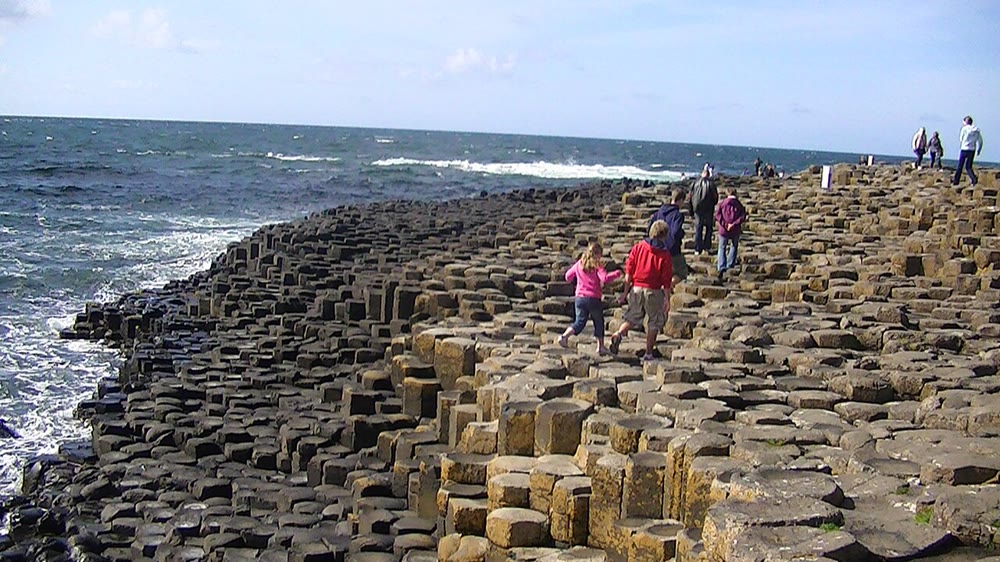
\includegraphics[height=4.3cm]{images/book2/g11-bishop-giants-causeway.jpg}\hspace{0.04\linewidth}%
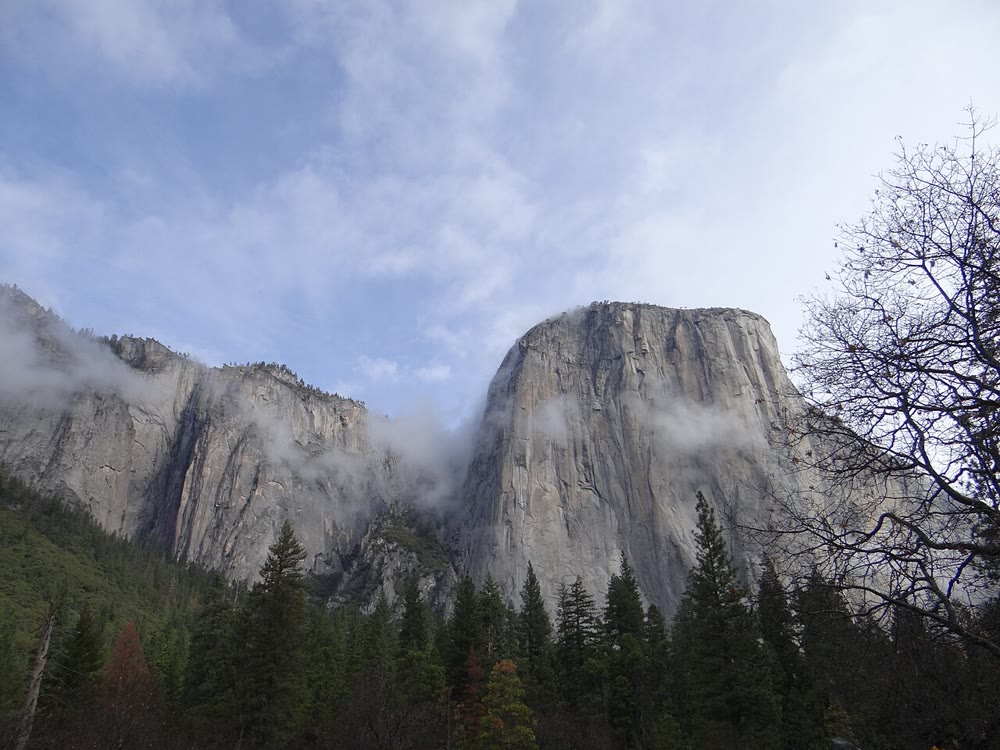
\includegraphics[height=4.3cm]{images/book2/g11-usgs-el-capitan.jpg}

{\small 左：巨人堤道的玄武岩柱，北爱尔兰。
照片：Adam Bishop（CC~BY-SA~3.0）。右：酋长岩，优胜美地，
加利福尼亚州，高约 \qty{900}{m} 的花岗岩峭壁。照片：
U.S. Geological Survey（CC0）。}
\end{omfigure}
% ledger: photo:g11-giants-causeway, photo:g11-el-capitan

\begin{recall}
岩浆是地表之下的熔融岩石；它喷出地表时成为熔岩，可以平缓流出，
也可以猛烈爆发（第 1 册，七年级）。火成岩是熔融岩石
冷却凝固形成的岩石（第 1 册，六年级）。玄武岩是一种暗色的\omterm{def:g11:igneous-rocks:volcanic-plutonic}{火山岩}，花岗岩则是
由长石、石英和云母组成的浅色岩石（第 1 册，六年级）。地幔
\omterm{def:g11:ocean-ridges:peridotite}{橄榄岩}在上升至洋脊之下时部分熔化，形成\omterm{def:g11:ocean-ridges:oceanic-lithosphere}{洋壳}中的玄武岩和
\omterm{def:g11:ocean-ridges:gabbro}{辉长岩}（见\cref{ch:g11:ocean-ridges}）。\omterm{def:g11:minerals:rock-forming}{造岩硅酸盐}
有橄榄石、辉石、角闪石、云母、长石和石英；
长石包括钾长石和斜长石，二者构成一个系列，
由富钙端元过渡到富钠端元（见\cref{ch:g11:minerals}）。热量以
热传导方式扩散，扩散距离约为 $\sqrt{\kappa t}$（$t$ 为时间），
其中 $\kappa$ 为热扩散率（见\cref{ch:g11:subduction-zones}）。
\end{recall}
% ledger: tulane:ridge-rocks, england:kelvin

\section{火山岩与深成岩}

\begin{definition}[火山岩；深成岩]\label{def:g11:igneous-rocks:volcanic-plutonic}
由岩浆结晶形成的火成岩，
若岩浆在地表以熔岩形式凝固，则称为\emph{火山岩}\index{火山岩}
（或喷出岩）；若岩浆在地下深处、
于其他岩石之中结晶，则称为\emph{深成岩}\index{深成岩}
（或侵入岩）。
\end{definition}
% ledger: tulane:magma-types

两者的差别体现在晶体大小上。晶体通过不断吸收周围液体中的
原子而生长，这需要时间。在地表，
熔岩很快将热量散失到空气或水中：喷入空气或水中的物质
数秒即可冷却，熔岩流则需数天至数周。在地下深处，
周围岩石温度高，岩浆散热缓慢：浅层\omterm{def:g11:igneous-rocks:intrusion}{侵入体}
需数月至数年冷却，大型\omterm{def:g11:igneous-rocks:intrusion}{深成岩体}可能需要数百万
年。快速冷却形成许多细小晶体，甚至没有晶体；缓慢冷却则
形成的晶体较少，但要大得多。
% ledger: tulane:cooling-times, tulane:textures

\begin{definition}[结构]\label{def:g11:igneous-rocks:texture}
岩石的\emph{结构}\index{结构（岩石的）}是指其颗粒的大小、形状
与排列方式。火成岩若不含晶体，则称为\emph{玻璃质}的；
若晶体细小到肉眼无法分辨，则称为\emph{细粒}的；
若晶体都可用肉眼看见，则称为
\emph{粗粒}的。
\end{definition}
% ledger: tulane:textures

熔岩在晶体来得及生长之前急速冷却，便形成玻璃：黑曜石，黑色
且呈玻璃质，\omterm{def:g11:minerals:cleavage}{断口}呈瓶子那样的贝壳状。玄武岩
为细粒岩石：手持标本时无法辨认其中的矿物，即使在
\omterm{def:g11:minerals:thin-section}{薄片}中，晶体也很小（即\cref{ch:g11:minerals}中的玄武岩）。
花岗岩、\omterm{def:g11:ocean-ridges:gabbro}{辉长岩}和\omterm{def:g11:igneous-rocks:rock-names}{闪长岩}为粗粒岩石：每一颗粒都清晰可见。
% ledger: photo:g11-obsidian, photo:g11-basalt, tulane:textures

\begin{definition}[斑晶；斑状]\label{def:g11:igneous-rocks:porphyritic}
嵌在大量细小晶体或玻璃中的大晶体称为\emph{斑晶}\index{斑晶}，
这些细小晶体或玻璃构成的整体称为\emph{基质}。含斑晶的岩石
称为\emph{斑状}\index{斑状}岩石。
\end{definition}
% ledger: tulane:textures

\omterm{def:g11:igneous-rocks:porphyritic}{斑状}\omterm{def:g11:igneous-rocks:texture}{结构}记录了两个冷却阶段：先是缓慢冷却，发生在地下深处，
此时\omterm{def:g11:igneous-rocks:porphyritic}{斑晶}在仍以液相为主的岩浆中生长；随后
快速冷却，岩浆上升喷出，或侵入到冷岩石中，
剩余的液体凝固成基质。
% ledger: tulane:textures

\begin{omfigure}
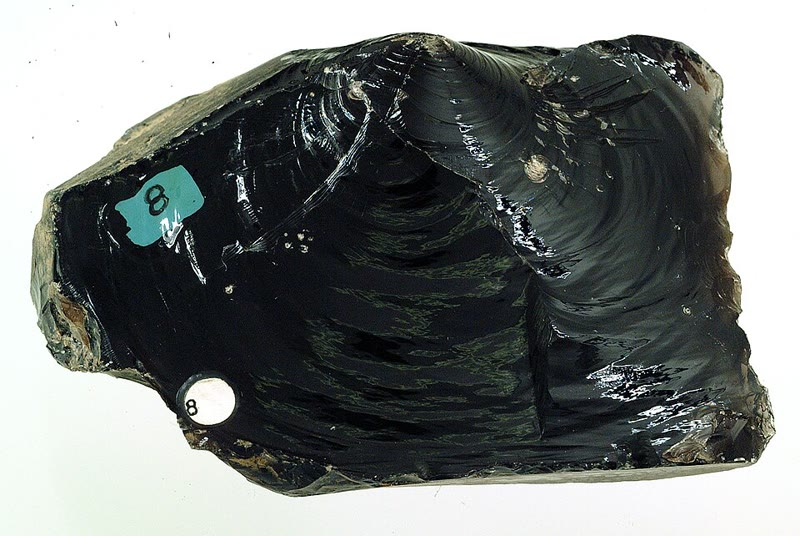
\includegraphics[height=2.75cm]{images/book2/g11-geodil-obsidian.jpg}\hfill
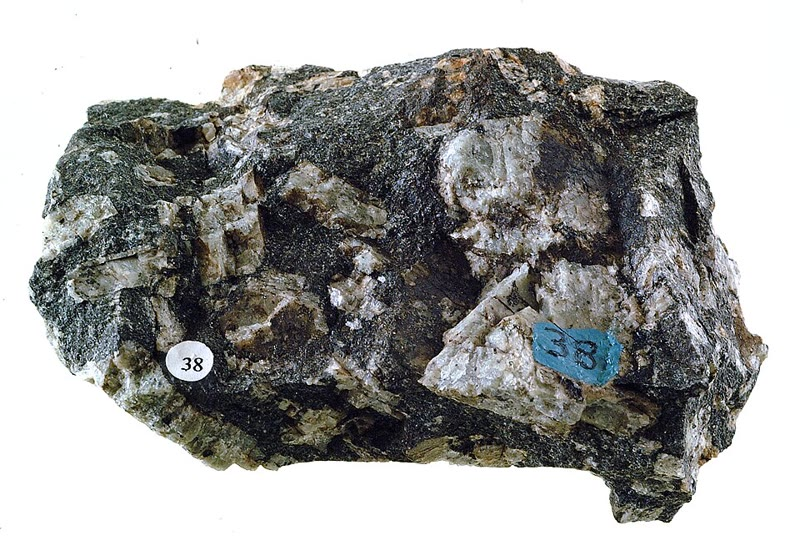
\includegraphics[height=2.75cm]{images/book2/g11-geodil-diabase-porphyry.jpg}\hfill
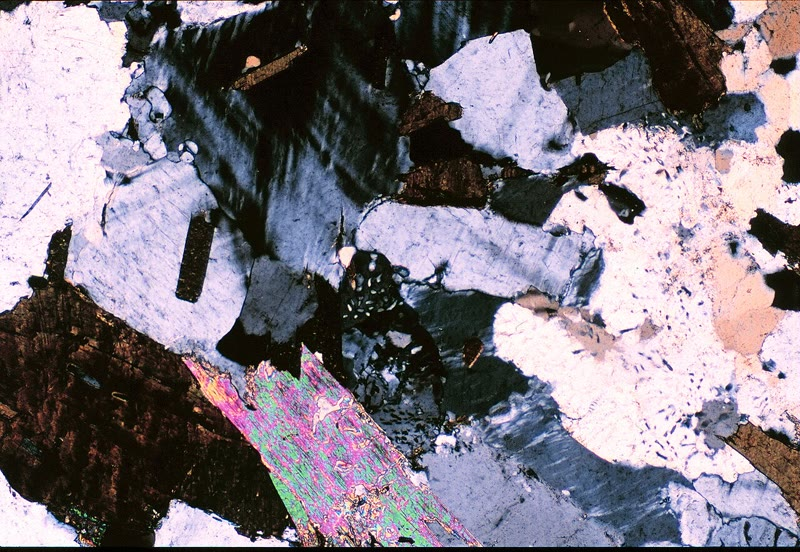
\includegraphics[height=2.75cm]{images/book2/g11-geodil-granite-xpl.jpg}\hfill
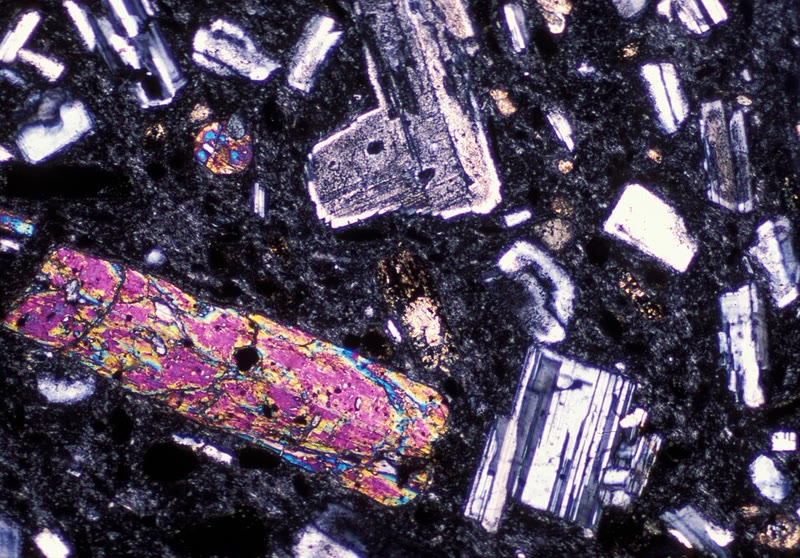
\includegraphics[height=2.75cm]{images/book2/g11-geodil-andesite-xpl.jpg}

{\small 从左到右：黑曜石，一种火山玻璃，其弯曲的
贝壳状\omterm{def:g11:minerals:cleavage}{断口}（直径 \qty{9.5}{cm}）；一块\omterm{def:g11:igneous-rocks:porphyritic}{斑状}岩石，块状的
斜长石\omterm{def:g11:igneous-rocks:porphyritic}{斑晶}嵌在较细的基质中（\qty{9}{cm}）；然后是两幅
正交偏光下的\omterm{def:g11:minerals:thin-section}{薄片}：花岗岩，所有颗粒均大且相互嵌合——
棕色黑云母、色彩鲜艳的白云母、条纹状的
斜长石、灰色和白色的石英；\omterm{def:g11:igneous-rocks:rock-names}{安山岩}，\omterm{def:g11:igneous-rocks:porphyritic}{斑晶}为
斜长石和角闪石，嵌在细粒基质中。照片：Twyla
Baker、Mike Davis 与 Darla Sondrol，Geology Digital Image Library（CC0）。}
\end{omfigure}
% ledger: photo:g11-obsidian, photo:g11-diabase-porphyry, photo:g11-granite-xpl, photo:g11-andesite-xpl

\section{命名火成岩}

火成岩的第二个判别依据是其化学成分，尤其是其
二氧化硅含量，即 \ce{SiO2}，在常见岩浆中
约占质量的 \qty{45}{\percent} 至 \qty{75}{\percent}。

\begin{definition}[镁铁质；中性；长英质]\label{def:g11:igneous-rocks:felsic-mafic}
岩浆或其形成的岩石，若为\emph{镁铁质}\index{镁铁质}，则
含 \qty{45}{\percent} 至 \qty{55}{\percent} 的 \ce{SiO2}，且富含铁、镁和钙；
为\emph{中性}\index{中性（岩石）}，其含量介于
\qty{55}{\percent} 与 \qty{65}{\percent} 之间；为\emph{长英质}\index{长英质}，则
含 \qty{65}{\percent} 至 \qty{75}{\percent} 的 \ce{SiO2}，
贫铁、镁和钙而富含钠和钾。
\end{definition}
% ledger: tulane:magma-types, earle:magma-oxides

每种岩浆可形成两种岩石：一种是细粒的\omterm{def:g11:igneous-rocks:volcanic-plutonic}{火山岩}，另一种是
粗粒的\omterm{def:g11:igneous-rocks:volcanic-plutonic}{深成岩}，二者化学成分相同。玄武岩与\omterm{def:g11:ocean-ridges:gabbro}{辉长岩}构成\omterm{def:g11:igneous-rocks:felsic-mafic}{镁铁质}的一对，
见于\omterm{def:g11:ocean-ridges:oceanic-lithosphere}{洋壳}；花岗岩则是\omterm{def:g11:igneous-rocks:felsic-mafic}{长英质}的\omterm{def:g11:igneous-rocks:volcanic-plutonic}{深成岩}。
另有三个名称补全了这一组。

\begin{definition}[安山岩；闪长岩；流纹岩]\label{def:g11:igneous-rocks:rock-names}
\emph{安山岩}\index{安山岩}与\emph{闪长岩}\index{闪长岩}分别是
\omterm{def:g11:igneous-rocks:felsic-mafic}{中性}成分的\omterm{def:g11:igneous-rocks:volcanic-plutonic}{火山岩}与\omterm{def:g11:igneous-rocks:volcanic-plutonic}{深成岩}，主要由
斜长石与角闪石或辉石组成。\emph{流纹岩}\index{流纹岩}是
\omterm{def:g11:igneous-rocks:felsic-mafic}{长英质}成分的\omterm{def:g11:igneous-rocks:volcanic-plutonic}{火山岩}，是花岗岩的
细粒对应岩石。
\end{definition}
% ledger: tulane:magma-types, earle:bowen, photo:g11-andesite, photo:g11-diorite

\begin{omfigure}
\begin{tikzpicture}[font=\footnotesize, x=0.4cm]
  % columns: SiO2 45 to 75 % mapped to x = 45 to 75 (0.4 cm per %)
  \begin{scope}[xshift=-18cm]
  \fill[omLithBasalt!45] (45,0) rectangle (55,2.4);
  \fill[omLithBasalt!20] (55,0) rectangle (65,2.4);
  \fill[omLithGranite!45] (65,0) rectangle (75,2.4);
  \draw[black!60] (45,0) rectangle (75,2.4);
  \draw[black!60] (55,0) -- (55,2.4); \draw[black!60] (65,0) -- (65,2.4);
  \draw[black!60] (45,1.2) -- (75,1.2);
  \foreach \x/\a/\b in {50/玄武岩/辉长岩, 60/安山岩/闪长岩, 70/流纹岩/花岗岩}{
    \node[font=\small\bfseries, text height=1.6ex, text depth=0.3ex] at (\x,1.8) {\a};
    \node[font=\small\bfseries, text height=1.6ex, text depth=0.3ex] at (\x,0.6) {\b};}
  \node[anchor=east, align=right] at (44.4,1.8) {细粒 \\（火山）};
  \node[anchor=east, align=right] at (44.4,0.6) {粗粒 \\（深成）};
  \node[anchor=south] at (50,2.45) {镁铁质};
  \node[anchor=south] at (60,2.45) {中性};
  \node[anchor=south] at (70,2.45) {长英质};
  % minerals (a drawing: where each mineral is common)
  \foreach \y/\a/\b/\m/\c in {-0.55/45.2/52/橄榄石/omLithBasalt!80!black,
      -1.15/45.2/61/辉石/omLithBasalt!65!black,
      -1.75/52/69/角闪石/black!60,
      -2.35/57/74.8/黑云母/black!75,
      -2.95/45.2/72/斜长石/omDef!45,
      -3.55/63/74.8/钾长石/omLithGranite!90!red,
      -4.15/64/74.8/石英/black!20,
      -4.75/68/74.8/白云母/black!35}{
    \fill[\c] (\a,\y) .. controls ({\a+1.2},{\y+0.22}) and ({\b-1.2},{\y+0.22}) .. (\b,\y)
              .. controls ({\b-1.2},{\y-0.22}) and ({\a+1.2},{\y-0.22}) .. (\a,\y) -- cycle;
    \node[anchor=east] at (44.4,\y) {\m};}
  \node[font=\scriptsize, text=black!75] at (50,-2.95) {富钙};
  \node[font=\scriptsize, text=omDef!80!black, anchor=west] at (72.3,-2.95) {富钠};
  % SiO2 axis
  \draw[-{Stealth[length=4pt]}] (45,-5.35) -- (75.8,-5.35);
  \foreach \x in {45,50,...,75} {\draw (\x,-5.35) -- (\x,-5.45); \node[anchor=north] at (\x,-5.45) {\x};}
  \node[anchor=north] at (60,-5.85) {\ce{SiO2}（\unit{\percent}，按质量计）};
  \draw[black!30, dashed] (55,0) -- (55,-5.35); \draw[black!30, dashed] (65,0) -- (65,-5.35);
  \end{scope}
\end{tikzpicture}

{\small 常见火成岩的命名（示意图）。列：岩浆的二氧化硅
含量；行：细粒（火山）岩与粗粒（深成）岩。下方标出
各造岩矿物的常见位置：橄榄石与辉石见于\omterm{def:g11:igneous-rocks:felsic-mafic}{镁铁质}岩，
伴有富钙的斜长石；角闪石与斜长石见于\omterm{def:g11:igneous-rocks:felsic-mafic}{中性}岩；
钾长石、石英、富钠的斜长石及云母
见于\omterm{def:g11:igneous-rocks:felsic-mafic}{长英质}岩。界线是
渐变的。}
\end{omfigure}
% ledger: tulane:magma-types, earle:bowen, earle:magma-oxides, photo:g11-andesite, photo:g11-diorite, photo:g11-granite, nps:granite-minerals

\begin{method}[火成岩的命名]\label{met:g11:igneous-rocks:naming}
\begin{enumerate}
  \item 观察\omterm{def:g11:igneous-rocks:texture}{结构}：玻璃质、细粒或粗粒；
        是否\omterm{def:g11:igneous-rocks:porphyritic}{斑状}。细粒或玻璃质表示\omterm{def:g11:igneous-rocks:volcanic-plutonic}{火山岩}（或
        快速冷却的小型\omterm{def:g11:igneous-rocks:intrusion}{侵入体}）；粗粒则表示\omterm{def:g11:igneous-rocks:volcanic-plutonic}{深成岩}。
  \item 识别可见的矿物
        （见\cref{met:g11:minerals:identify}）：石英与钾长石
        指示\omterm{def:g11:igneous-rocks:felsic-mafic}{长英质}，角闪石与斜长石指示\omterm{def:g11:igneous-rocks:felsic-mafic}{中性}，橄榄石
        与辉石指示\omterm{def:g11:igneous-rocks:felsic-mafic}{镁铁质}。在细粒岩石中，可参考\omterm{def:g11:igneous-rocks:porphyritic}{斑晶}、
        基质的颜色——深色指示\omterm{def:g11:igneous-rocks:felsic-mafic}{镁铁质}，浅色指示\omterm{def:g11:igneous-rocks:felsic-mafic}{长英质}——
        作为提示，或借助化学分析。
  \item 读取图中行与列交叉处的
        岩石名称。
\end{enumerate}
\end{method}

\begin{example}[两种玄武岩]
取自熔岩流的一块暗色岩石通体为细粒；另一块来自同一火山，
在暗色基质中可见直径数毫米的绿色橄榄石颗粒。两者均为
\omterm{def:g11:igneous-rocks:felsic-mafic}{镁铁质}且为细粒，故都是玄武岩。第二块是\omterm{def:g11:igneous-rocks:porphyritic}{斑状}玄武岩：
其橄榄石先在火山下方的岩浆中缓慢生长，
之后熔岩喷出并在其周围凝固。
\end{example}
% ledger: photo:g11-olivine, earle:bowen, tulane:textures

\begin{omfigure}
\makebox[0.32\linewidth]{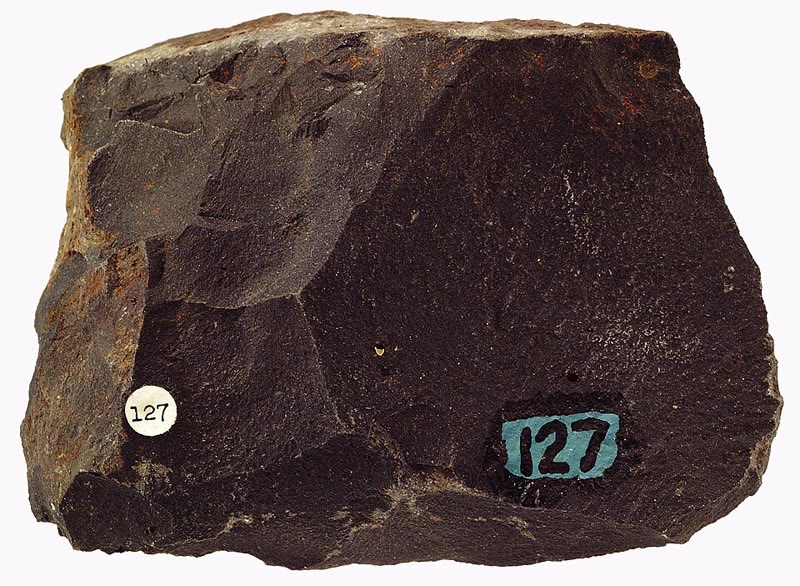
\includegraphics[height=2.9cm]{images/book2/g11-geodil-basalt.jpg}}\hfill
\makebox[0.32\linewidth]{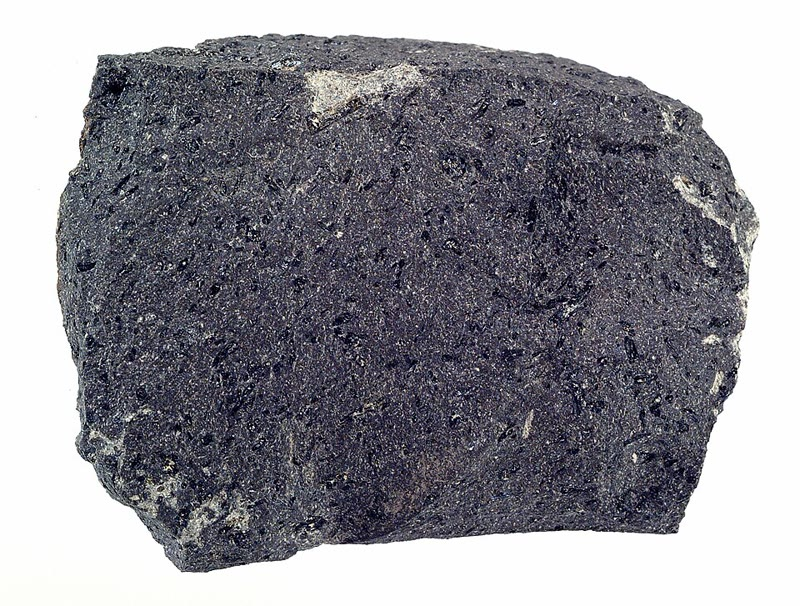
\includegraphics[height=2.9cm]{images/book2/g11-geodil-andesite.jpg}}\hfill
\makebox[0.32\linewidth]{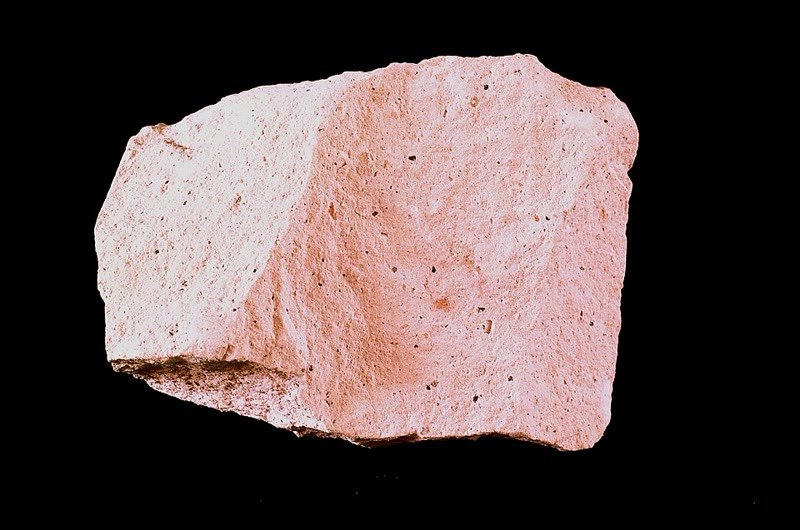
\includegraphics[height=2.9cm]{images/book2/g11-geodil-rhyolite.jpg}}

\smallskip
\makebox[0.32\linewidth]{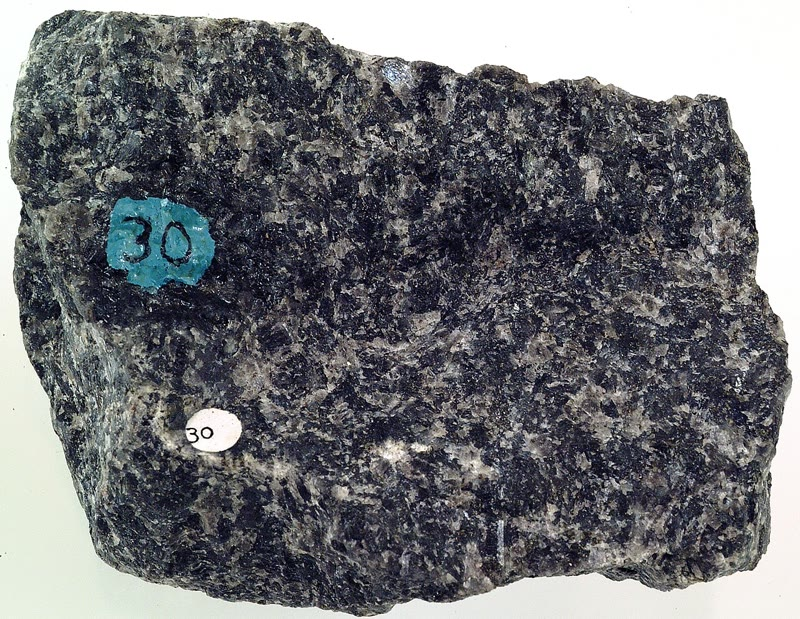
\includegraphics[height=2.9cm]{images/book2/g11-geodil-gabbro.jpg}}\hfill
\makebox[0.32\linewidth]{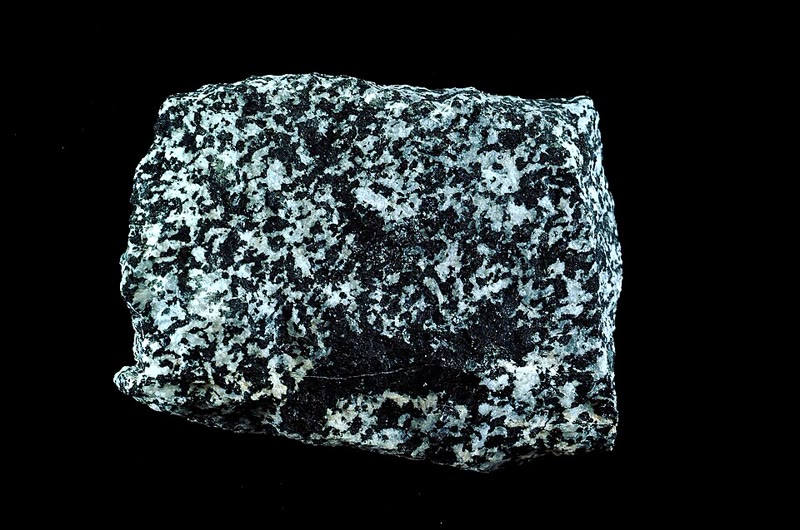
\includegraphics[height=2.9cm]{images/book2/g11-geodil-diorite.jpg}}\hfill
\makebox[0.32\linewidth]{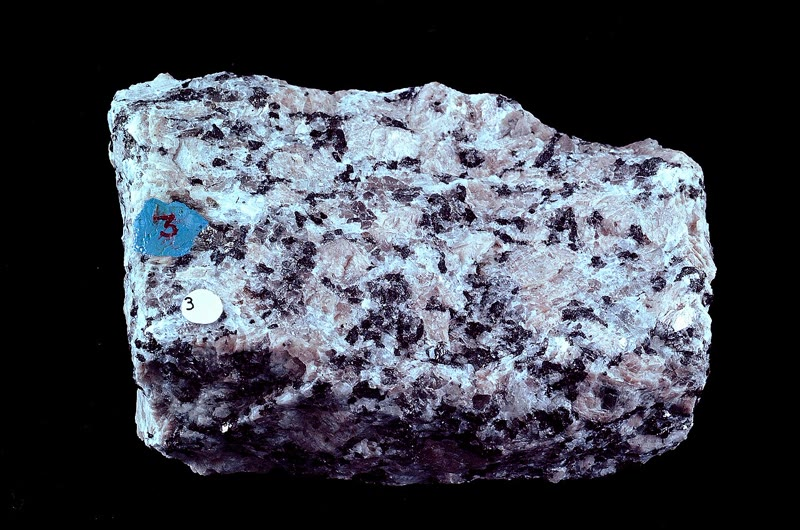
\includegraphics[height=2.9cm]{images/book2/g11-geodil-granite.jpg}}

{\small 从左到右依次为三对由\omterm{def:g11:igneous-rocks:felsic-mafic}{镁铁质}到\omterm{def:g11:igneous-rocks:felsic-mafic}{长英质}的火成岩：
上排为\omterm{def:g11:igneous-rocks:volcanic-plutonic}{火山岩}，下排为\omterm{def:g11:igneous-rocks:volcanic-plutonic}{深成岩}。上排：细粒玄武岩；\omterm{def:g11:igneous-rocks:rock-names}{安山岩}，
细小的角闪石晶体散布于细粒基质中（约 \qty{10}{cm}）；
粉红色的\omterm{def:g11:igneous-rocks:rock-names}{流纹岩}。下排：\omterm{def:g11:ocean-ridges:gabbro}{辉长岩}（\qty{9}{cm}）；\omterm{def:g11:igneous-rocks:rock-names}{闪长岩}，黑色角闪石与
玻璃质斜长石（\qty{10}{cm}）；粗粒花岗岩，含大块浅粉色
钾长石、灰色斜长石、石英、黑云母与角闪石。
（\qty{10}{cm}）。照片：Nessa Eull、Twyla Baker、Joseph H.~Hartman、
Darla Sondrol 与 Dexter Perkins，Geology Digital Image Library（CC0）。}
\end{omfigure}
% ledger: photo:g11-basalt, photo:g11-andesite, photo:g11-rhyolite, photo:g11-gabbro, photo:g11-diorite, photo:g11-granite

\section{结晶顺序}

岩浆并不像水那样在单一温度下凝固。其中的矿物
随冷却依次出现，各自有其特定的温度范围，
因此冷却中的岩浆可以既含晶体，又仍以液体为主。

\begin{history}[鲍文的实验]
诺曼·L.~鲍文（1887--1956）于 1912 年加入
华盛顿卡内基研究所地球物理实验室。他主要研究玄武质
岩浆：在炉中熔化岩石，使其缓慢冷却至选定温度，
使部分矿物生成，随后将其骤冷，冷却得如此之快，
以致剩余液体凝为玻璃。在显微镜下，
晶体显示了哪些矿物是在该温度以上形成的。逐次降低温度重复实验，
实验由此给出各矿物出现的
先后次序。鲍文于 1922 年将此次序以反应系列的形式发表，
并于 1928 年出版专著\emph{The Evolution of the Igneous Rocks}。
\end{history}
% ledger: carnegie:bowen, earle:bowen

\begin{omfigure}
\begin{tikzpicture}[font=\footnotesize, box/.style={draw=black!60, rounded corners=2pt, fill=#1, minimum width=3.0cm, minimum height=0.62cm, align=center}]
  \node[box=omLithBasalt!45] (ol) at (0,0) {橄榄石};
  \node[box=omLithBasalt!35] (px) at (0,-1.1) {辉石};
  \node[box=black!15] (am) at (0,-2.2) {角闪石};
  \node[box=black!25] (bi) at (0,-3.3) {黑云母};
  \draw[-{Stealth[length=4pt]}, line width=0.8pt] (ol) -- (px);
  \draw[-{Stealth[length=4pt]}, line width=0.8pt] (px) -- (am);
  \draw[-{Stealth[length=4pt]}, line width=0.8pt] (am) -- (bi);
  \node[align=center, anchor=south] at (0,0.45) {\textbf{不连续分支}\\每种矿物与液体反应 \\生成下一种};
  % continuous branch: a wedge from Ca-rich to Na-rich
  \fill[left color=omDef!55, right color=omDef!12, shading angle=180] (5.0,-0.9) -- (6.6,-0.9) -- (6.6,-3.5) -- (5.0,-3.5) -- cycle;
  \shade[top color=omDef!60, bottom color=omDef!10, draw=black!60, rounded corners=2pt] (4.3,-0.85) rectangle (7.3,-3.55);
  \node[align=center] at (5.8,-1.3) {富钙 \\斜长石};
  \node[align=center] at (5.8,-3.15) {富钠 \\斜长石};
  \draw[-{Stealth[length=4pt]}, line width=0.8pt] (5.8,-1.65) -- (5.8,-2.7);
  \node[align=center, anchor=south] at (5.8,0.45) {\textbf{连续分支}\\斜长石 \\逐渐变化};
  % last minerals
  \node[box=omLithGranite!45, minimum width=7.6cm] (last) at (2.9,-4.75) {钾长石、石英、（白云母）};
  \draw[-{Stealth[length=4pt]}, line width=0.8pt] (bi) -- (bi |- last.north);
  \draw[-{Stealth[length=4pt]}, line width=0.8pt] (5.8,-3.55) -- (5.8,-4.43);
  % temperature arrow
  \draw[-{Stealth[length=5pt]}, line width=1pt, omThm] (-2.6,0.3) -- (-2.6,-4.9);
  \node[anchor=east, align=right, text=omThm] at (-2.75,0.1) {最初，\\\qtyrange{1200}{1300}{\degreeCelsius}};
  \node[anchor=east, align=right, text=omThm] at (-2.75,-4.7) {最后，约 \\\qtyrange{750}{800}{\degreeCelsius}};
  \node[anchor=east, align=right, text=omThm] at (-2.75,-2.3) {温度 \\下降};
\end{tikzpicture}

{\small 矿物从冷却岩浆中结晶的先后顺序
（鲍文反应系列，示意图）。橄榄石最先形成；斜长石开始结晶的位置
大致与辉石相当，起初富钙，之后
钠含量越来越高。钾长石、石英以及有时出现的
白云母最后形成，由富硅残余液体结晶而成。}
\end{omfigure}
% ledger: earle:bowen

其中\emph{反应}一词很关键。橄榄石仅在高温下稳定：
岩浆冷却时，橄榄石晶体与液体中的二氧化硅反应，
转变为辉石，
\[
  \ce{Mg2SiO4 + SiO2 -> 2 MgSiO3},
\]
沿此分支依此类推，只要液体中仍有二氧化硅。沿另一分支，
斜长石晶体持续生长，但每一新生层
都比前一层更富钠：斜长石晶体可以呈环带\omterm{def:g11:igneous-rocks:texture}{结构}，由富钙的
核心逐渐过渡到富钠的边缘，与上方\omterm{def:g11:igneous-rocks:rock-names}{安山岩}中的斜长石
\omterm{def:g11:igneous-rocks:porphyritic}{斑晶}相似。
% ledger: earle:bowen, photo:g11-andesite-xpl

反应系列可以解释上图。\omterm{def:g11:igneous-rocks:felsic-mafic}{镁铁质}岩浆较早耗尽二氧化硅：它
结晶出橄榄石、辉石与富钙斜长石，若缓慢冷却于地下
便形成\omterm{def:g11:ocean-ridges:gabbro}{辉长岩}；若在地表快速冷却，则形成玄武岩。只有富硅的
岩浆才能进行到系列末端，
形成钾长石与石英：即花岗岩与\omterm{def:g11:igneous-rocks:rock-names}{流纹岩}的矿物。
岩浆在此过程中成分如何变化，即早期晶体与液体分离时，
属于本科二年级的内容。
% ledger: earle:bowen, tulane:bowen

\section{侵入体}

岩浆上升，是因为其密度小于周围岩石，它挤入
裂隙并使之扩大。岩浆大部分从未抵达地表：
它在地壳中结晶，形成\omterm{def:g11:igneous-rocks:intrusion}{侵入体}，只有在
上覆岩石被侵蚀掉之后才能看到。
% ledger: tulane:intrusions

\begin{definition}[岩墙；岩床；深成岩体]\label{def:g11:igneous-rocks:intrusion}
称\emph{侵入体}\index{侵入体}为在其他岩石内部
结晶形成的火成岩体。称\emph{岩墙}\index{岩墙}为
一种切穿所侵入岩石层理或\omterm{def:g11:igneous-rocks:texture}{结构}的火成岩板状体；
而\emph{岩床}\index{岩床}则是平行于
岩层之间的板状体。称\emph{深成岩体}\index{深成岩体}为
形成于较大深度、形状任意的大型侵入体；许多\omterm{def:g11:igneous-rocks:volcanic-plutonic}{深成岩}体
相连则形成岩基（见\cref{ch:g12:subduction-magmatism}）。
\end{definition}
% ledger: tulane:intrusions

\omterm{def:g11:igneous-rocks:intrusion}{岩墙}通常宽不足 \qty{20}{m}，\omterm{def:g11:igneous-rocks:intrusion}{岩床}通常厚不足 \qty{50}{m}；
\omterm{def:g11:igneous-rocks:intrusion}{岩床}通常由\omterm{def:g11:igneous-rocks:intrusion}{岩墙}供给岩浆。浅层的\omterm{def:g11:igneous-rocks:intrusion}{岩墙}与\omterm{def:g11:igneous-rocks:intrusion}{岩床}冷却很快：
它们是细粒的，有时呈\omterm{def:g11:igneous-rocks:porphyritic}{斑状}。
岩浆侵入冷岩石时，其边缘冷却最快，
比中心还要细粒：这种边缘称为\emph{冷凝边}，是岩体就位时仍然炽热的标志。
位于加利福尼亚州、约塞米蒂所在之处的内华达山脉，
是一座岩基：其密度已在\cref{ch:g11:minerals}中测定的花岗质岩石，
即来自其中约两百个\omterm{def:g11:igneous-rocks:intrusion}{深成岩体}。
% ledger: tulane:intrusions, usgs91:sierra, photo:g11-el-capitan

\begin{omfigure}
\begin{tikzpicture}[font=\footnotesize, scale=0.9]
  % layered host rocks
  \fill[omLithSand] (0,0) rectangle (14,-1.0);
  \fill[omLithShale] (0,-1.0) rectangle (14,-2.0);
  \fill[omLithLime] (0,-2.0) rectangle (14,-3.0);
  \fill[omLithSand] (0,-3.0) rectangle (14,-4.0);
  \fill[omLithShale] (0,-4.0) rectangle (14,-6.4);
  \foreach \y in {-1,-2,-3,-4} \draw[black!35] (0,\y) -- (14,\y);
  % pluton
  \fill[omLithGranite, draw=black!60] (2.2,-6.4) .. controls (2.4,-4.6) and (3.6,-4.1) .. (5.5,-4.15)
     .. controls (7.4,-4.2) and (9.0,-4.5) .. (9.6,-6.4) -- cycle;
  % sill between the limestone and the shale, fed by the dyke
  \fill[omLithBasalt, draw=black!60] (7.3,-1.88) -- (12.6,-1.88) .. controls (12.9,-1.9) and (12.9,-2.1) .. (12.6,-2.12) -- (7.3,-2.12) -- cycle;
  % dyke from the pluton to the volcano
  \fill[omLithBasalt, draw=black!60] (7.0,-4.18) -- (7.3,-4.2) -- (7.3,0) -- (7.0,0) -- cycle;
  % a second dyke cutting across the layers, not reaching the surface
  \fill[omLithBasalt, draw=black!60] (3.9,-4.15) -- (4.15,-4.15) -- (2.95,-0.6) -- (2.75,-0.6) -- cycle;
  % volcano and lava flow
  \fill[black!65] (5.75,0) -- (7.15,1.35) -- (8.55,0) -- cycle;
  \fill[omLithBasalt!80!black] (8.4,0) -- (11.6,0) -- (11.6,0.1) .. controls (10.5,0.16) and (9.2,0.22) .. (8.3,0.15) -- cycle;
  \draw[black!70] (0,0) -- (5.75,0); \draw[black!70] (8.55,0) -- (14,0);
  % labels
  \node[anchor=south] at (7.15,1.4) {火山};
  \draw[black!60] (10.5,0.15) -- (11.2,0.8); \node[anchor=south west, inner sep=1pt] at (11.2,0.8) {熔岩流};
  \draw[black!60] (7.3,-0.5) -- (8.3,-0.5); \node[anchor=west, fill=omLithSand, inner sep=1pt] at (8.3,-0.5) {岩墙（切穿岩层）};
  \draw[black!60] (11.0,-2.0) -- (11.0,-2.55); \node[anchor=north, fill=omLithLime, inner sep=1pt] at (11.0,-2.55) {岩床（位于岩层之间）};
  \draw[black!60] (3.4,-2.5) -- (1.9,-2.5); \node[anchor=east, fill=omLithLime, inner sep=1pt] at (1.9,-2.5) {岩墙};
  \node[align=center] at (5.9,-5.5) {深成岩体};
  \node[anchor=east, fill=omLithShale, inner sep=1pt] at (13.85,-5.3) {层状沉积岩};
\end{tikzpicture}

{\small \omterm{def:g11:igneous-rocks:intrusion}{侵入体}示意图（非按比例绘制）。\omterm{def:g11:igneous-rocks:intrusion}{深成岩体}在深处结晶；
\omterm{def:g11:igneous-rocks:intrusion}{岩墙}切穿其上方岩层的层理，其中一条为一座
火山供给岩浆；\omterm{def:g11:igneous-rocks:intrusion}{岩床}展布于两层岩层之间。只有上覆岩层被侵蚀，
这些岩体才会出露于地表。}
\end{omfigure}
% ledger: tulane:intrusions

\omterm{def:g11:igneous-rocks:intrusion}{侵入体}需要多长时间才能结晶？考虑一块
厚度为 $b$ 的岩浆板——\omterm{def:g11:igneous-rocks:intrusion}{岩墙}或\omterm{def:g11:igneous-rocks:intrusion}{岩床}——通过
向两侧岩石的传导散失热量。决定进程快慢的量只有
是厚度 $b$（单位为米）和热扩散率 $\kappa$，
单位为 \unit{m^2/s}；由它们能构成的唯一时间尺度是 $b^2/\kappa$。
% ledger: england:kelvin, delaney86:example

\begin{proposition}[岩浆板的冷却时间]\label{prop:g11:igneous-rocks:cooling}
厚度为 $b$ 的岩浆板若通过传导冷却，
则凝固所需的时间为
\[
  t = C\,\frac{b^2}{\kappa},
\]
其中 $\kappa$ 为岩石的热扩散率，$C$ 为由岩浆与周围岩石的
温度，以及岩浆结晶时释放的热量
所决定的数，将厚度加倍，
则时间变为四倍。（在本阶段不加证明地承认；$C$ 的值由计算模型给出。）
\end{proposition}
% ledger: delaney86:properties, delaney86:example

玄武质岩浆以 \qty{1150}{\degreeCelsius} 侵入
温度为 \qty{50}{\degreeCelsius} 的岩石中，完全结晶的温度为
\qty{950}{\degreeCelsius}，每结晶一立方米释放 \qty{900}{MJ} 的热量。
取 $\kappa = \qty{1e-6}{m^2/s}$，模型给出
$C \approx 0.21$。厚 \qty{2}{m} 的岩浆板约需十天凝固，
厚 \qty{20}{m} 的\omterm{def:g11:igneous-rocks:intrusion}{岩床}约需两年半，而
厚 \qty{100}{m} 的则约需六十五年。若不计结晶释放的热量，
时间将缩短为原来的三分之一：结晶中的岩浆
会自行保温。
% values (dyke_cooling.py): t2_day 9.55, t20_yr 2.61, t100_yr 65.3, latent_factor 2.94; C = 8.2475e7 s / 4e8 s = 0.206
% ledger: delaney86:example, delaney86:properties, england:kelvin

\begin{omfigure}
\begin{tikzpicture}
\begin{axis}[omrecord, name=times, width=0.45\linewidth, height=5.0cm, xmode=log, ymode=log,
  xmin=0.8, xmax=130, ymin=1e-3, ymax=200, xlabel={岩浆板厚度（\unit{m}）},
  ylabel={凝固所需时间（年）},
  legend style={font=\scriptsize, at={(0.5,-0.4)}, anchor=north, legend columns=2,
    /tikz/every even column/.append style={column sep=4pt}}]
% computed in figdata/grade-11/dyke_cooling.py; ledger: delaney86:*, england:kelvin
\addplot[omThm, line width=1pt, mark=*, mark size=1.4pt] table[x=b, y=t_yr] {figdata/out/grade-11-dyke_cooling-times.dat};
\addplot[omDef, line width=1pt, dashed, mark=o, mark size=1.4pt] table[x=b, y=t0_yr] {figdata/out/grade-11-dyke_cooling-times.dat};
\legend{计入结晶热, 不计入}
\end{axis}
\begin{axis}[omrecord, at={(times.east)}, anchor=west, xshift=1.6cm, width=0.45\linewidth, height=5.0cm,
  xmin=-28, xmax=28, ymin=0, ymax=1300, xlabel={距岩床中心的距离（\unit{m}）},
  ylabel={温度（\unit{\degreeCelsius}）},
  legend style={font=\scriptsize, at={(0.5,-0.4)}, anchor=north, legend columns=4,
    /tikz/every even column/.append style={column sep=4pt}}]
\fill[omLithBasalt!30] (axis cs:-10,0) rectangle (axis cs:10,1300);
\draw[black!50, dashed] (axis cs:-28,950) -- (axis cs:28,950);
\node[font=\scriptsize, anchor=south east, text=black!60] at (axis cs:27,955) {固相线};
\node[font=\scriptsize, anchor=north] at (axis cs:0,1290) {岩床};
% computed in figdata/grade-11/dyke_cooling.py
\addplot[omProp, line width=0.9pt] table[x=x, y=T1] {figdata/out/grade-11-dyke_cooling-profiles.dat};
\addplot[omThm, line width=0.9pt] table[x=x, y=T2] {figdata/out/grade-11-dyke_cooling-profiles.dat};
\addplot[omDef, line width=0.9pt] table[x=x, y=T3] {figdata/out/grade-11-dyke_cooling-profiles.dat};
\addplot[black, line width=0.9pt] table[x=x, y=T4] {figdata/out/grade-11-dyke_cooling-profiles.dat};
\legend{30 天, 6 个月, 1 年, 2 年}
\end{axis}
\end{tikzpicture}

{\small 一层玄武岩质岩浆以传导方式冷却（计算模型）。
左图：凝固所需时间与厚度的关系，采用对数坐标，
坐标轴上为斜率 2 的直线，即凝固时间随
厚度的平方增长。右图：厚 \qty{20}{m} 的\omterm{def:g11:igneous-rocks:intrusion}{岩床}内的温度分布（阴影部分），
以 \qty{1150}{\degreeCelsius} 的温度侵入
\qty{50}{\degreeCelsius} 的围岩中。边缘立即降至固相线以下，
中心则约两年半后才降到固相线以下。}
\end{omfigure}
% values (dyke_cooling.py): profiles at 30, 180, 365, 730 days; contact about 690 degC (Delaney: 690)

模型还显示出冷凝边的形成。接触面处的岩石
立即升至约 \qty{690}{\degreeCelsius}，远低于固相线：
\omterm{def:g11:igneous-rocks:intrusion}{岩床}最初几厘米在一天内即凝固，而其中心
则数年内保持液态。实际\omterm{def:g11:igneous-rocks:intrusion}{侵入体}要复杂得多——岩石性质随温度变化，
地下水会循环，\omterm{def:g11:igneous-rocks:intrusion}{深成岩体}位于本已很热的岩石中，
并可能反复得到补给——这就是为什么大型深部\omterm{def:g11:igneous-rocks:intrusion}{侵入体}
的冷却时间远长于冷主岩条件下定律所预示的，
这一点并不意外。
% ledger: delaney86:example, tulane:cooling-times
% values (dyke_cooling.py): margin_day_20m 0.58 (cell 12.5 cm from the contact)

\section{练习}

\begin{exercise}[$\star$]\label{exo:g11:igneous-rocks:1}
定义\omterm{def:g11:igneous-rocks:volcanic-plutonic}{火山岩}与\omterm{def:g11:igneous-rocks:volcanic-plutonic}{深成岩}。给出三对成分相同的\omterm{def:g11:igneous-rocks:volcanic-plutonic}{火山岩}与\omterm{def:g11:igneous-rocks:volcanic-plutonic}{深成岩}，
按从\omterm{def:g11:igneous-rocks:felsic-mafic}{镁铁质}到\omterm{def:g11:igneous-rocks:felsic-mafic}{长英质}的顺序排列。
\end{exercise}

\begin{exercise}[$\star$]\label{exo:g11:igneous-rocks:2}
将每种岩石与其\omterm{def:g11:igneous-rocks:texture}{结构}配对——玻璃质、细粒、粗粒、
\omterm{def:g11:igneous-rocks:porphyritic}{斑状}：（1）黑曜岩；（2）花岗岩；（3）玄武岩，含直径数毫米的绿色
橄榄石晶体，嵌于深色基质中；（4）玄武岩，其中
肉眼无法辨认出任何矿物。
\end{exercise}

\begin{exercise}[$\star$]\label{exo:g11:igneous-rocks:3}
三种岩浆中 \ce{SiO2} 的含量分别为 \qty{48}{\percent}、\qty{60}{\percent} 和
\qty{72}{\percent}。分别对其分类，并说出每种岩浆
在深部缓慢冷却时形成的岩石名称。
\end{exercise}

\begin{exercise}[$\star$]\label{exo:g11:igneous-rocks:4}
定义\omterm{def:g11:igneous-rocks:intrusion}{岩墙}、\omterm{def:g11:igneous-rocks:intrusion}{岩床}和\omterm{def:g11:igneous-rocks:intrusion}{深成岩体}。在本章的\omterm{def:g11:igneous-rocks:intrusion}{侵入体}示意图中，
哪一个\omterm{def:g11:igneous-rocks:intrusion}{侵入体}为火山提供了岩浆？
\end{exercise}

\begin{exercise}[$\star$]\label{exo:g11:igneous-rocks:5}
在鲍文反应序列中，哪种矿物最先形成，哪些矿物
最后形成？斜长石在岩浆冷却时如何变化？
\end{exercise}

\begin{exercise}[$\star\star$]\label{exo:g11:igneous-rocks:6}
对两种岩石进行分析（质量百分比）。岩石 A：\ce{SiO2} 74，\ce{Al2O3}
14，\ce{FeO} 3，\ce{CaO} 3，\ce{MgO} 0.5，\ce{Na2O} 5，\ce{K2O} 4。岩石 B：
\ce{SiO2} 47，\ce{Al2O3} 14，\ce{FeO} 8，\ce{CaO} 10，\ce{MgO} 8，\ce{Na2O}
1，\ce{K2O} 2。（1）分别对其分类。（2）用其余氧化物检验你的答案。
（3）岩石 A 为细粒\omterm{def:g11:igneous-rocks:texture}{结构}，请给出其名称；岩石 B 为粗粒\omterm{def:g11:igneous-rocks:texture}{结构}，
亦请给出其名称。
\end{exercise}

\begin{exercise}[$\star\star$]\label{exo:g11:igneous-rocks:7}
厚 \qty{2}{m} 的\omterm{def:g11:igneous-rocks:intrusion}{岩墙}约十天凝固。利用
关于冷却时间的命题，同种岩浆形成的\omterm{def:g11:igneous-rocks:intrusion}{岩墙}若厚
\qty{1}{m}，需要多长时间？厚 \qty{20}{m} 的\omterm{def:g11:igneous-rocks:intrusion}{岩床}呢？厚 \qty{200}{m} 的呢？
\end{exercise}

\begin{exercise}[$\star\star$]\label{exo:g11:igneous-rocks:8}
（1）证明 $b^2/\kappa$ 是一个时间。（2）计算 $b = \qty{20}{m}$ 时的值，
$\kappa = \qty{1e-6}{m^2/s}$，分别以秒和年为单位
（$\num{1}\text{ 年} \approx \qty{3.16e7}{s}$）。（3）取 $C = 0.21$，
\omterm{def:g11:igneous-rocks:intrusion}{岩床}需要多长时间才能凝固？
\end{exercise}

\begin{exercise}[$\star\star$]\label{exo:g11:igneous-rocks:9}
一块岩石中可见块状斜长石晶体，长约一厘米，
基质中的颗粒肉眼无法分辨。描述其\omterm{def:g11:igneous-rocks:texture}{结构}，并分两个阶段
叙述其冷却历程。
\end{exercise}

\begin{exercise}[$\star\star$]\label{exo:g11:igneous-rocks:10}
橄榄石与液相中的二氧化硅反应：$\ce{Mg2SiO4 + SiO2 -> 2
MgSiO3}$。（1）检验该方程式是否配平。（2）已知摩尔质量
\qty{140.7}{g/mol}（\ce{Mg2SiO4}）和 \qty{60.1}{g/mol}（\ce{SiO2}），
则 \qty{1}{kg} 橄榄石从液相中夺取的二氧化硅质量为多少？（3）为什么
二氧化硅含量低的岩浆仍能保留其橄榄石？
\end{exercise}

\begin{exercise}[$\star\star$]\label{exo:g11:igneous-rocks:11}
厚 \qty{20}{m}、面积为 \qty{1}{m^2} 的\omterm{def:g11:igneous-rocks:intrusion}{岩床}，
由 \qty{1150}{\degreeCelsius} 冷却至 \qty{50}{\degreeCelsius}。（1）其热容为
每立方米每摄氏度 \qty{2.5}{MJ}，冷却时损失多少热量？
（2）结晶时每立方米还释放 \qty{900}{MJ} 的热量，
其值为多少？（3）比较两者。
\end{exercise}

\begin{exercise}[$\star\star\star$]\label{exo:g11:igneous-rocks:12}
在厚 \qty{20}{m} \omterm{def:g11:igneous-rocks:intrusion}{岩床}的计算模型中，距接触面
\qty{12.5}{cm} 处的岩石约经过
\num{0.6}~天后降到固相线以下，距接触面 \qty{5}{m} 处的岩石约经过 545 天，
中心约经过 950 天。（1）你认为\omterm{def:g11:igneous-rocks:intrusion}{岩床}中何处晶体最小，何处最大？
（2）固体层生长的速率是否恒定？
（3）为什么\omterm{def:g11:igneous-rocks:intrusion}{岩床}即使在中心处也是细粒\omterm{def:g11:igneous-rocks:texture}{结构}，
与花岗岩相比？
\end{exercise}

\begin{exercise}[$\star\star\star$]\label{exo:g11:igneous-rocks:13}
\omterm{def:g11:igneous-rocks:intrusion}{深成岩体}厚 \qty{2}{km}。（1）利用上述命题及
\qty{20}{m} \omterm{def:g11:igneous-rocks:intrusion}{岩床}（约 2.6 年）的数据，估算其冷却时间。（2）大型深部\omterm{def:g11:igneous-rocks:intrusion}{侵入体}
已知其冷却可长达数百万年。试给出两条理由，
说明为何简单定律低估了冷却时间。
\end{exercise}

\begin{exercise}[$\star\star\star$]\label{exo:g11:igneous-rocks:14}
\omterm{def:g11:igneous-rocks:felsic-mafic}{长英质}岩浆的喷发温度约为 \qtyrange{650}{800}{\degreeCelsius}，\omterm{def:g11:igneous-rocks:felsic-mafic}{镁铁质}
岩浆约为 \qtyrange{1000}{1200}{\degreeCelsius}。试利用鲍文
反应系列，解释花岗岩为何含有钾长石、石英
和富钠斜长石而不含橄榄石，而\omterm{def:g11:ocean-ridges:gabbro}{辉长岩}含有橄榄石、
辉石和富钙斜长石，而不含石英。
\end{exercise}

\begin{exercise}[$\star\star\star$]\label{exo:g11:igneous-rocks:15}
喷入空气中的物质数秒内即冷却，熔岩流需数天至数周，
浅层\omterm{def:g11:igneous-rocks:intrusion}{侵入体}需数月至数年。（1）利用命题，约一天凝固的岩层
厚度为多少？（2）一层厚 \qty{5}{m} 的熔岩流
约一个月凝固，这是否符合两侧冷却板状体的定律？
（3）各种情形下预期会出现何种\omterm{def:g11:igneous-rocks:texture}{结构}？
\end{exercise}

\section{问题：岩床及其晶体}

\begin{problem}[{周末问题——岩床凝固需要多长时间}]
\label{pb:g11:igneous-rocks:1}
% values (dyke_cooling.py): t20_yr 2.61, margin_day_20m 0.58, t2_day 9.55, contact ~690 degC;
% C = 0.206; ledger delaney86:*, tulane:*, earle:*
在某山谷的岩壁中，有一层厚 \qty{20}{m} 的深色火成岩板状体，
夹于两层砂岩之间，与之平行。自
其边缘至中心采集样品。接触带处岩石极细粒，几近
玻璃质；距边缘 \qty{1}{m} 处，晶体约 \qty{0.1}{mm}；在
中心处约 \qty{1}{mm}，斜长石与辉石可
用手持放大镜勉强区分。

\medskip
\noindent\textbf{第一部分——岩石\omterm{def:g11:igneous-rocks:texture}{结构}。}
\begin{enumerate}
  \item 该板状体是\omterm{def:g11:igneous-rocks:intrusion}{岩墙}还是\omterm{def:g11:igneous-rocks:intrusion}{岩床}？为什么？
  \item 描述接触带与中心处的\omterm{def:g11:igneous-rocks:texture}{结构}。
  \item 为何接触带处的岩石晶粒最细？
  \item 这种细粒边缘称为什么，它对板状体
        就位时的温度说明了什么？
  \item 该\omterm{def:g11:igneous-rocks:intrusion}{岩床}由下方一条同种岩石的竖直板状体供给，
        厚 \qty{2}{m}，切穿砂岩。它是什么？
\end{enumerate}

\medskip
\noindent\textbf{第二部分——岩石命名。}
\begin{enumerate}[resume]
  \item 一项分析给出 \qty{49}{\percent} \ce{SiO2}、\qty{10}{\percent}
        \ce{FeO}、\qty{7}{\percent} \ce{MgO} 和 \qty{10}{\percent}
        \ce{CaO}。该岩浆是\omterm{def:g11:igneous-rocks:felsic-mafic}{镁铁质}、\omterm{def:g11:igneous-rocks:felsic-mafic}{中性}还是\omterm{def:g11:igneous-rocks:felsic-mafic}{长英质}？
  \item 据鲍文系列，你预期会出现哪些矿物？
  \item 接触带岩石应定名为何？哪种\omterm{def:g11:igneous-rocks:volcanic-plutonic}{深成岩}具有
        与之相同的成分？
  \item 同一岩浆体为何能形成\omterm{def:g11:igneous-rocks:texture}{结构}不同的岩石？
  \item 橄榄石、辉石和斜长石开始结晶的
        先后顺序如何？
\end{enumerate}

\medskip
\noindent\textbf{第三部分——冷却时间。}
\begin{enumerate}[resume]
  \item 计算\omterm{def:g11:igneous-rocks:intrusion}{岩床}的 $b^2/\kappa$，取 $\kappa = \qty{1e-6}{m^2/s}$，
        结果以秒为单位。
  \item 模型给出 $C = 0.206$。计算\omterm{def:g11:igneous-rocks:intrusion}{岩床}凝固所需的时间，以
        秒为单位，再以年为单位（$\num{1}\text{ 年} \approx \qty{3.16e7}{s}$）。
  \item 厚 \qty{2}{m} 的供给板状体需要多长时间凝固？
  \item 若不计结晶热，$C$ 约为 $0.07$。
        \omterm{def:g11:igneous-rocks:intrusion}{岩床}需要多长时间？为何结晶会减缓
        冷却？
  \item 模型给出距接触带 \qty{12.5}{cm} 处的岩石约需 \num{0.6}~天
        凝固。与中心相比，它快了
        多少倍？
\end{enumerate}

\medskip
\noindent\textbf{第四部分——晶体提供的信息。}
\begin{enumerate}[resume]
  \item 熔岩流在数天至数周内冷却，浅层\omterm{def:g11:igneous-rocks:intrusion}{侵入体}需数月至
        数年。该\omterm{def:g11:igneous-rocks:intrusion}{岩床}应归入哪一类？
  \item 晶体达一厘米或以上的花岗岩，冷却
        得慢得多。利用该定律估算，冷却时间
        为\omterm{def:g11:igneous-rocks:intrusion}{岩床}一千倍的板状体厚度为多少？
  \item 此类岩体为何必然形成于地壳深部？
  \item 今天\omterm{def:g11:igneous-rocks:intrusion}{岩床}出露于地表。其上覆岩石
        必然经历了怎样的变化？
  \item 综合以上结果，\omterm{def:g11:igneous-rocks:intrusion}{岩床}凝固用了多长时间？
\end{enumerate}
\end{problem}
